\chapter{Linear Algebra}

\section{Singular Value Decomposition} \label{sec:SVD}
Being able to diagonalize a matrix makes a lot of matrix manipulations a lot easier. Life becomes particularly easy if the transform used to diagonalize a matrix is orthogonal. The SVD provides an orthonormal diagonal decomposition for arbitrary (non-square) matrices. The catch: the basis vectors used for the domain/range can be different. So the SVD isn't necessarily suitable for applications with powers of matrices since you don't get $A^2 = S \Lambda S^\T S \Lambda S^\T = S \Lambda^2 S^\T$. But in a lot of other applications, it's very useful. 

Let $A\in \R^{m\times n}$ and let $r = \myrank{A}$. We want orthonormal bases $v_1,\ldots, v_r$  for the row space and $u_1,\ldots,u_r$ for the column space such that
$$
A v_i = \sigma_i u_i
$$
for some $\sigma_i \in \R$, $i=1,\ldots, r$. 
What is a good candidate for $(v_i)_{i=1}^r$ and $(u_i)_{i=1}^f$? How about the eigenvectors of  $A^\T A \in \R^{n\times n}$ and $AA^\T\in \R^{m\times m}$? These matrices are symmetric positive semidefinite. To verify PSD, note that $x^\T A^\T A x = \|A^\T x\|^2 \geq 0 ~ \forall x$. Because these matrices are symmetric, they have an orthogonal set of eigenvectors. This is an immediate consequence of the spectral theorem--see Exercise \ref{exer:spectral_thrm}. Let $(v_i)_{i=1}^r$ be orthonormal eigenvectors of $A^\T A$ with associated eigenvalues given by $\sigma_i^2$. Note that
$$
A^\T Av_i = \sigma_i^2 v_i \implies  v_i^\T A^\T A v_i = \sigma_i^2 v_i^\T v_i \implies \|A v_i\| = \sigma_i.
$$
Now, let $u_i := \frac{1}{\sigma_i}Av_i$. By the previous display, $u_i$ is a unit vector. Ideally, we would like the set of $Av_i$ to map to an orthonormal basis in the column space. Let's see what happens. We have
$$
A^\T A v_i = \sigma_i^2 v_i \iff AA^\T Av_i = \sigma_i^2 A v_i \iff A A^\T v_i = \sigma_i^2 u_i. 
$$
So, $u_i = \frac{1}{\sigma_i} A v_i$ is a unit eigenvector of $A A^\T$. Thus, we have
\begin{itemize}
  \item $(u_i)_{i=1}^r$ is an orthonormal basis for the column space
  \item $(v_i)_{i=1}^r$ is an orthonormal basis for the row space
  \item $Av_i = \sigma u_i$
  \item $\sigma_i \geq 0$, $\sigma_i = \sqrt{\lambda_i}$ where $\lambda_i \in \sigma(A^\T A)$
\end{itemize}
Now, complete each basis with orthonormal basis for the the nullspace and left nullspace of $A$ to get $(v_1,\ldots,v_r,\ldots, v_n)$ and $(u_1,\ldots, u_r, \ldots, u_m)$. Let $V\in \R^{n\times n}$ be formed columnwise from $(v_i)_i$ and likewise form $U\in \R^{m\times m}$ columnwise from $(u_i)_i$. Let $\Sigma \in \R^{m\times n}$ be formed by placing $\sigma_i$ on the diagonal. Of course, do this all with a consistent ordering so eigenvectors and eigenvalues in each matrix match. We have
$$
A v_i = \sigma_i u_i \iff AV = U\Sigma \iff \underbrace{A =  U \Sigma V^\T}_{\text{SVD}}
$$
This last expression is the SVD. The columns of $U$ and $V$ are known, respectively, as the left and right singular vectors of $A$ and $(\sigma_i)$ are the singular values. 

%\subsection{Examples and Applications?}
%\myred{TODO}: Add another section here building intuition about anything? Like, how should you think about singular values? Just as orthogonal scaling factors when mapping to the new basis? Anything useful to think about with relationship between singular values and eigenvalues?
%
%Stuff I'd like to cover somewhere:
%\begin{itemize}
%  \item low rank approximation
%  \item connections to PCA
%  \item connections to pseudo inverse (next) and then connections to linear regression
%\end{itemize}


\section{Pseudo Inverse} \label{sec:pseudo-inv}

For a linear mapping $A$, $\row A$ and $\col A$ have the same dimension (see Exercise \ref{exer:rank-transpose-eqal}). This seems like a remarkable fact.
The linear mapping $A$ is a bijection between $\row A$ and $\col A$ (see Exercise \ref{exer:restricted-bijection} for the full rank case).\footnote{\myred{TODO}: Full case?} The pseudo-inverse, denoted by $A^+$, maps from $\col A$ back to $\row A$. That is, for an element $\y$ in $\col A$, $A^+\y$ recovers the unique $\x$ in $\row A$ such that $A \x = \y$. If $\y\in (\col A)^{\perp} = N(A^\T)$, then $A^{+}\y=0$. The pseudo-inverse coincides with $A^{-1}$ when it exists. 

Figure \ref{fig:pseudo-inv}, taken from a Gilbert Strang paper, clearly illustrates the action of $A^+$. 

\begin{figure} \label{fig:pseudo-inv}
\centering
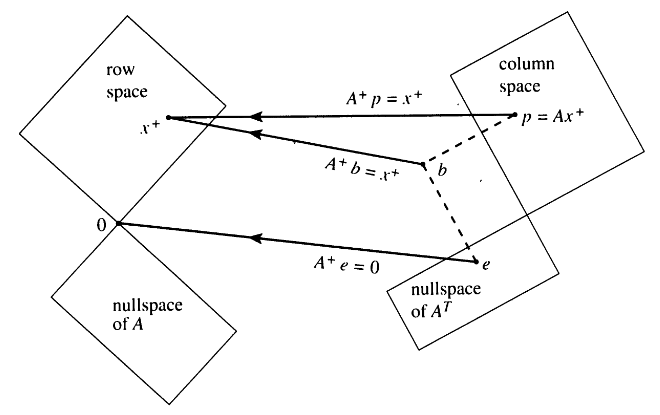
\includegraphics[scale = .5]{/least_squares/pseudo-inv}
\caption{Action of pseudo-inverse (taken from Strang paper).}
\end{figure}

The matrix $A^+$ satisfying these properties can be clearly derived from the SVD. Let $\myrank A = r$, and let $(u_i)_{i=1}^r$ and $(v_i)_{i=1}^r$ be as defined in Section \ref{sec:SVD}, so that these are orthonormal bases of the column and row spaces respectively. We have $Av_i = \sigma u_i$. We would like an inverse satisfying 
$$
A^+ \sigma u_i = v_i \iff A^+ u_i = \frac{1}{\sigma_i} v_i \iff A^+ U = V\Sigma^+
$$
where $\Sigma^+$ is the same dimensions as $\Sigma^\T$, but with $1/\sigma_i$ on the diagonal where $\sigma_i \not= 0$ holds by definition since we only define $\sigma_i$ up to $r=\myrank A$. 
Hence, the pseudo-inverse is given by 
\begin{equation}
A^+ = V\Sigma^+ U^\T
\end{equation}

\myred{TODO}: There are a couple of important subtleties I'm missing here. What to do with zero singular values? What's the dimension of $\Sigma$. Just lock that down and be consistent. Also, order $\sigma_1 \geq \cdots \geq \sigma_r > 0$

\section{Low-Rank Matrix Approximation}
\noindent \textbf{Problem Statement}
Let $A\in \R^{m\times n}$ be a real matrix with $m< n$ and let $d$ be a positive integer that will be used to represent a rank constraint. We would like to find a matrix $A_d$ satisfying 
\begin{align}
A_d \in & \arg\min_{B\in \R^{m\times n}} \|A - B\|\\
\mbox{s.t. } ~ & \myrank{B} \leq d.
\end{align}
Note that we have not been specific about the precise norm used. The solution can vary based on the norm used (I think). But we'll see that the optimal solution follows readily from the SVD when we use the Frobenius or spectral norm. 

\begin{theorem}
Let $A = U\Sigma V^\T$ be the SVD of $A$. Let $U_d\in \R^{m\times d}$ and $V_d\in \R^{n\times d}$ be the matrices constructed from the first $d$ columns of $U$ and $V$, where we assume the convention that $\Sigma$ is ordered as in ??. 
Then
$$
A_d := U_r \Sigma_d V_d^\T
$$
is an optimal rank $d$ approximation in the sense that
$$
\|A - A_d\|_F \leq \|A - B\|_F \quad \mbox{ and } \quad \|A - A_d\|_2 \leq \|A - B\|_2 \quad \forall B \mbox{ s.t. } \myrank{B} \leq d.
$$
\end{theorem}

\myred{TODO} Add in proof for Frobenius norm. Can use Weyl's inequality. See \href{https://en.wikipedia.org/wiki/Weyl\%27s_inequality}{here} and link to Tao notes therein. Also, might be nice to spend some time looking at variational expression for eigenvalues and applications. Or can use a different proof from \href{https://people.math.osu.edu/costin.10/5101/Low\%20rank\%20Approx.pdf}{here}.

\section{Important Matrix Decompositions}
\myred{TODO}: Cholesky, QR. Applications to numerical linear algebra. 

%\section{Possible sections}
%\begin{itemize}
%\item Any important facts about eigenvalues?
%\item Unitary matrices (these are actually important) 
%\item Normal matrices? (What are these useful for? I get that the properties seem important. But I haven't really run into them in my work. Maybe skip for now unless I really feel like it.) 
%\item Schur complement
%\end{itemize}


\section{Exercises}
%%
\begin{exercise} \label{exer:rank-transpose-eqal}
  Let $A\in M_{m,n}$. Show $\myrank A = \myrank A^\T$.
\end{exercise}

\begin{solution}
  This actually feels like a moderately deep result. Can prove using RREF, which seems unpleasant. Or using Steinitz exchange lemma. See \href{https://en.wikipedia.org/wiki/Rank_(linear_algebra)#Proof_using_linear_combinations}{here}.
\end{solution}

%%
\begin{exercise}
  Show $\row A \perp N(A)$.
\end{exercise}

\begin{solution}
Immediate from the definitions. $x\in N(A) \implies Ax = 0 \implies x$ is orthogonal to every row of $A$, which implies that it is orthogonal to any linear combination of rows. 
\end{solution}
  
%%
\begin{exercise}
\textbf{Rank-nullity theorem.} For $A\in \R^{m\times n}$, show that $\myrank A + \dim N(A) = n$.
\end{exercise}

\begin{solution}
Proof on Wiki is pretty simple. Construct a basis for $N(A)$. Extend this to a full basis of $\R^n$. Call the basis $S$. Now, take $B = S\backslash N(A)$. Show that $\text{im} A = \myspan S$ (easy). Show that $A(S)$ is in fact a basis for $\text{im} A$. (You'd expect this based on a dimensionality counting argument. But we don't know the dimension of im$A$ yet. So, just verify that it's a basis. We've already shown $\myspan A(S) = \text{im}(A)$. Now just show that the set $A(S)$ is linearly independent. Just verify the definition of linear independence. 
\end{solution}

%%
\begin{exercise} \label{exer:spectral_thrm}
\textbf{Spectral theorem.} Show that if $A$ is Hermitian (or just real symmetric for an easier version) that $A$ may be decomposed as $A = Q\Lambda Q^T$, where $Q$ is orthonormal and $\Lambda$ is diagonal. 
\end{exercise}

\begin{solution}
\begin{proof}
For any real matrix $A$ and any vectors $x$ and $y$ we have
$$
\langle Ax, y\rangle = \langle x, A^\T y\rangle.
$$
Now assume that $A$ is symmetric and $x$ and $y$ are eigenvectors of $A$ corresponding to distinct eigenvalues $\lambda$ and $\mu$. Then 
$$
\lambda \langle x, y\rangle = \rangle \lambda x, y\rangle = \langle Ax, y\rangle = \langle x, A^\T y\rangle = \langle x, A y\rangle = \langle x, \mu y \rangle = \mu\langle x, y \rangle.
$$
Hence, $(\lambda - \mu)\langle x, y\rangle = 0$. Since $\lambda - \mu \not= 0$, then $\langle x, y\rangle = 0$, i.e., $x \perp y$. 
Now, find an orthonormal basis for each eigenspace. (If eigenvalues are unique, this is trivial. But if there are repeated eigenvalues, then you need to find an orthonormal basis for the eigenspace \myred{TODO}: How do you know the geometric multiplicity matches the algebraic multiplicity for each eigenvector? See \href{https://math.stackexchange.com/questions/393149/for-a-symmetric-matrix-the-geometric-and-algebraic-multiplicities-are-equal}{here}. ) Since eigenspaces are mutually orthogonal, these vectors together give an orthonormal subset of $\R^n$. Let $Q$ be the orthonormal matrix formed columnwise from these vectors $(v_i)_{i=1}^n$. The eigenvalue condition $Av_i = \lambda_i v_i$, $i=1,\ldots,n$ is equivalent to
$$
AQ = Q\Lambda. 
$$
Right multiplying both sides by $Q^\T$ gives the desired result. 
\end{proof}

Alternate proofs using variational characterization of eigenvalues \href{https://mmids-textbook.github.io/chap04_specgraph/03_extremal/roch-mmids-specgraph-extremal.html}{here} and \href{https://terrytao.wordpress.com/2010/01/12/254a-notes-3a-eigenvalues-and-sums-of-hermitian-matrices/}{here}
\end{solution}

%%
\begin{exercise}
Show that any symmetric matrix is diagonalizable.
\end{exercise}

\begin{solution}
Didn't follow this full \href{https://math.stackexchange.com/questions/482599/why-are-real-symmetric-matrices-diagonalizable}{solution}. 
\end{solution}

\begin{exercise}
A matrix $A$ is said to be diagonalizable if it is similar to a diagonal matrix. Show that a matrix $A$ is diagonalizable if and only if there is a set of $n$ linearly independent vectors, each of which is an eigenvector of $A$. 
\end{exercise}

\begin{solution}
Horn, matrix analysis, Theorem 1.3.7. 
\end{solution}

%%
\begin{exercise}
Singular values vs eigenvalues for symmetric matrices. Show the following: Suppose $A$ is a symmetric matrix. If $\lambda \in \sigma(A)$, then $\lambda^2 \in \sigma(A^\T A)$, and, in particular, $|\lambda |$ is an singular value of $A$. \\

Corollary: If $A$ is PSD, then the set of eigenvectors and singular values coincide. 
\end{exercise}

\begin{solution}
\myred{TODO}
\end{solution}

%
\begin{exercise}
Prove $\sigma(A) = \sigma(A^\T)$.
\end{exercise}

\begin{solution}
\end{solution}

% 
\begin{exercise} \label{exer:rank-eqs}
Show $\myrank X = \myrank X^\T X = \myrank X X^\T = \myrank X X^\T$. 
\end{exercise}

\begin{solution}
\begin{proof}
1. Claim that $\myrank X = \myrank X^\T$. This is a fundamental and moderately deep property of rank that can takes a little work to show. Skip the proof here. This should be an exercise in the Linear algebra chapter. 

2. Show that $X$ and $X^\T X$ have the same nullspace. Suppose $Xw = 0$. Then $X^\T Xw = 0$. So $N(X) \subset N(X^\T X)$. Now, suppose $X^\T X w = 0$. Then $w^\T X^\T X w = 0 \implies \|Xw\|^2 = 0 \implies Xw = 0 \implies w \in N(X)$. The result now follows by applying the rank-nullity theorem. Let $k = \dim N(X) = \dim N(X^\T X)$. Then the rank of either $X$ or $X^\T X$ is given by $n-k$.

Finally, the fact that $\myrank XX^\T = m$ follows from the fact that $\myrank A = \myrank A^\T$. 
\end{proof}
\end{solution}

%
\begin{exercise} \label{exer:restricted-bijection}
Suppose that $\hat y \in \col X$. Show there exists a unique $\hat w$ solving $X\hat w = \hat y$ (**). 
Prove above claim and compute $\hat w$ in terms of $X$ and $y$.\footnote{Note that this implies that, restricted to $\row X$, $X$ is injective to $\col X$. It's easy to show surjectivity to $\col X$, since $\col X$ is the range of $X$. For any $y\in \col X$, there exists a $\w$ s.t. $X\w = \y$. Use the fact that $\row X \perp N(X)$ to throw away the part of $\w\in N(X)$. Now you have a point $\w$ in $\row X$ that maps to $\y$.}
\end{exercise}

\begin{solution}
 $\myrank X^\T X = n \implies (X^\T X)^{-1}$ exists. Also, since $\hat y\in \col X$, a $\hat w$ solving (**) exists. Observe
 \begin{align}
 X \hat w = \hat y & \iff (X^\T X){-1} X^\T X\hat w = (X^\T X)^{-1} X^\T \hat y\\
 & \iff \hat w = (X^\T X)^{-1} X^\T \hat y
 \end{align}
 Also, we may verify that $N\left((X^\T X)^{-1} X^\T\right) = \{0\}$. This proves the claim. 
\end{solution}